\documentclass[10pt]{article}
\usepackage[letterpaper,margin=0.76in]{geometry}
\usepackage{graphicx,booktabs,tabularx,array,xcolor,microtype,enumitem,titlesec,caption,subcaption,fancyhdr,url,float}
\usepackage[hidelinks]{hyperref}
\graphicspath{{figures/}}

\definecolor{ink}{HTML}{17211C}
\definecolor{orange}{HTML}{E95F32}
\definecolor{blue}{HTML}{3E6FB5}
\definecolor{muted}{HTML}{66706A}
\definecolor{paper}{HTML}{F5F3ED}
\definecolor{rulegray}{HTML}{D6D6CF}
\hypersetup{colorlinks=true,linkcolor=ink,citecolor=blue,urlcolor=blue,
  pdftitle={Procedure Atlas: From HoloLens Recordings to Training-Ready Supervision},
  pdfauthor={AIOps Project}}
\titleformat{\section}{\large\bfseries\color{ink}}{\thesection}{0.55em}{}
\titleformat{\subsection}{\normalsize\bfseries\color{ink}}{\thesubsection}{0.55em}{}
\titlespacing*{\section}{0pt}{1.15em}{0.4em}
\titlespacing*{\subsection}{0pt}{0.8em}{0.22em}
\captionsetup{font=small,labelfont=bf,labelsep=period}
\setlist{nosep,leftmargin=1.35em}
\setlength{\parindent}{0pt}
\setlength{\parskip}{0.4em}
\setlength{\headheight}{20pt}
\renewcommand{\arraystretch}{1.14}
\newcolumntype{Y}{>{\raggedright\arraybackslash}X}
\newcommand{\code}[1]{\texttt{\small #1}}
\newcommand{\priority}[1]{\textbf{\color{orange}#1}}
\pagestyle{fancy}
\fancyhf{}
\fancyhead[L]{\small\color{muted}PROCEDURE ATLAS DATASET PROTOCOL}
\fancyhead[R]{\small\color{muted}AIOps Project}
\fancyfoot[C]{\small\color{muted}\thepage}
\renewcommand{\headrulewidth}{0.35pt}
\renewcommand{\headrule}{\hbox to\headwidth{\color{rulegray}\leaders\hrule height \headrulewidth\hfill}}

\begin{document}
\begin{titlepage}
\pagecolor{paper}
\vspace*{0.9cm}
{\small\bfseries\color{orange}DATASET METHODS REPORT \hfill JULY 2026}
\vspace{1.25cm}

{\fontsize{29}{33}\selectfont\bfseries\color{ink}
Procedure Atlas:\\From HoloLens Recordings to\\Training-Ready Supervision\par}
\vspace{0.45cm}
{\Large\color{muted}A general protocol for actions, execution mistakes,
hand pose, and optional multimodal evidence\par}
\vspace{1.0cm}

\noindent\colorbox{ink}{\parbox{\dimexpr\textwidth-2\fboxsep\relax}{
\vspace{0.55em}\color{white}\large
\textbf{Procedure Atlas / Multimodal Dataset Labeler}\\[-1pt]
\small ``Label the procedure. Ground the evidence.'' Human-in-the-loop
preparation of egocentric recordings for reproducible procedural learning.
\vspace{0.55em}}}

\vfill
\begin{tabularx}{\textwidth}{@{}>{\bfseries\color{ink}}p{0.23\textwidth}Y@{}}
Scope & HoloLens and first-person recordings; temporal actions; structured
mistakes; MediaPipe 21-landmark hands; optional object, tool, state, recovery,
and sensor-reference evidence.\\
Priority model & P0 is always on. P1 is optional, reversible, and may be disabled
when its evidence is unavailable.\\
Primary outputs & Project JSON, capture and temporal manifests, step and
hand-keypoint CSV, COCO keypoints, split files, procedure JSON, and YAML.\\
Document status & Operational protocol and research-paper-style system report.\\
\end{tabularx}
\vspace{0.85cm}

{\large\bfseries\color{ink}AIOps Project}\\
{\small\color{muted}Procedure Atlas schema 2.0 workflow}
\end{titlepage}
\nopagecolor

\begin{abstract}
Egocentric HoloLens recordings can support procedural action segmentation,
execution-error recognition, and hand-aware learning only when raw media is
converted into synchronized, auditable supervision. Procedure Atlas implements
an always-on P0 contract comprising capture identity and split metadata,
versioned action taxonomies, structured mistake semantics,
presentation-timestamp-based intervals, reviewable MediaPipe hand keyframes,
portable projects, and semantic validation. Optional P1 labeling adds overlapping
object/tool interaction, contact, task state, recovery, task-graph, and HoloLens
sensor-reference evidence. P1 is disabled by default and may be excluded from
exports without deleting saved optional annotations. Screenshots use a
20-second proxy extracted from the supplied
\code{20260716\_012249\_HoloLens.mp4}; their labels are illustrative, not
adjudicated ground truth. This report defines the operating procedure, release
gates, and remaining limitations for producing training-ready data.
\end{abstract}

\textbf{Keywords:} egocentric video; HoloLens; temporal action segmentation;
procedural errors; hand pose; multimodal evidence; dataset curation

\section{Objective and recommended identity}

\textbf{Recommended name: Procedure Atlas.} This is broader and more accurate
than ``Hand Atlas'' because the system labels a procedure, including its actions,
outcomes, hands, objects, tools, and state evidence. The recommended header is
\textbf{``Label the procedure. Ground the evidence.''} It communicates that
labels must be tied to observable or synchronized evidence, not inference.

Ego4D demonstrated the value of time-indexed wearable-camera data
\cite{grauman2022ego4d}; CaptainCook4D showed why procedural-error datasets need
both normal and erroneous executions \cite{peddi2024captaincook4d}. The target
dataset should support: (1) action recognition and segmentation, (2) structured
execution-error attribution, and (3) hand-aware learning. HoloLens Research Mode
can expose depth, tracking-camera, pose, and inertial streams
\cite{microsoft_research_mode}. The current app stores P1 references to such
streams but does not decode, calibrate, or synchronize them.

\section{Implemented system}

\subsection{P0: always-on training contract}

\begin{enumerate}
  \item \textbf{Identity and provenance:} participant, session, split, nominal
  frame rate, time base, annotator, reviewer, taxonomy version, and guideline
  version.
  \item \textbf{Temporal actions:} non-overlapping half-open intervals
  $[t_{\mathrm{start}},t_{\mathrm{end}})$ with stable class IDs; remaining time
  exports as \code{background}.
  \item \textbf{Structured outcomes:} incorrect segments require a mistake
  family, severity, expected and observed state, affected object, recovery
  action, and recoverability.
  \item \textbf{Hand pose:} MediaPipe proposes 21 landmarks per hand
  \cite{zhang2020mediapipe}; reviewers correct position and visibility before
  saving a human-reviewed keyframe.
  \item \textbf{Reproducibility:} autosave, undo/redo, portable save/open,
  editable segments, validation, and redundant exports.
\end{enumerate}

Presentation time in seconds is canonical. A browser-presented-frame counter is
separate; \code{source\_frame\_index} remains null unless an authoritative
decoder or manifest supplies it. Exported \code{z\_rel} is MediaPipe-relative
depth, not calibrated metric HoloLens depth.

\begin{figure}[H]
  \centering
  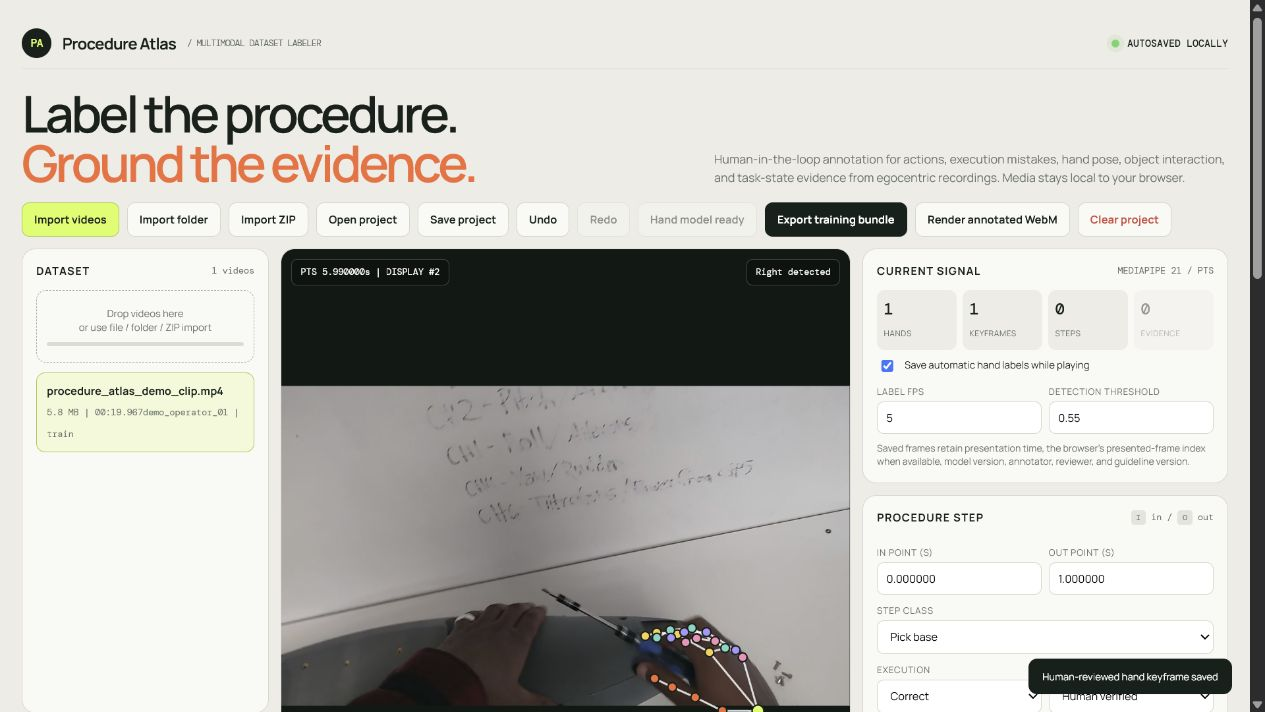
\includegraphics[width=\textwidth]{procedure_02_hand_overlay.png}
  \caption{Procedure Atlas on the supplied HoloLens demo dataset. The real
  egocentric frame shows a driver interaction and a detected right-hand
  21-joint overlay. The saved label is a workflow demonstration.}
  \label{fig:overview}
\end{figure}

\subsection{P1: optional evidence expansion}

P1 adds overlapping events for object interaction, tool use, task-state
transition, hand-object contact, recovery, and sensor anchors. Events can record
object/tool IDs, contact hand, pre/post-state, expected/observed effect,
confidence, and evidence notes. A task graph supports transition validation;
optional fields reference depth, gaze, head pose/IMU, calibration, and timing.

P1 is \textbf{off by default}. Disabling it preserves its records in the project
but excludes them from the training bundle. RGB-only datasets can therefore
produce complete P0 supervision without presenting unsupported P1 fields as
complete evidence.

\begin{figure}[H]
\centering
\begin{subfigure}[t]{0.48\textwidth}
  \centering
  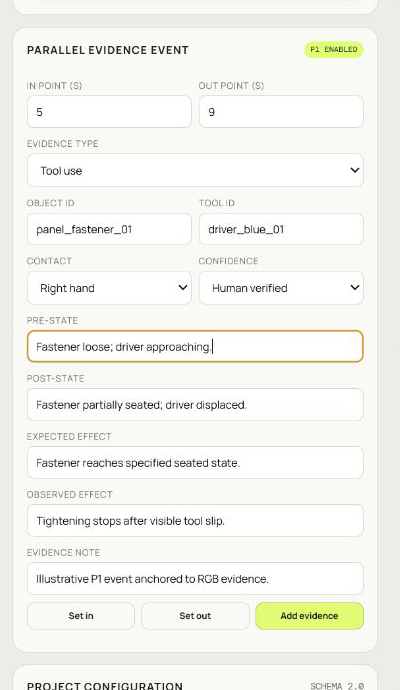
\includegraphics[height=0.34\textheight]{procedure_04_p1_optional.png}
  \caption{P1 enabled: overlapping tool-use evidence.}
\end{subfigure}\hfill
\begin{subfigure}[t]{0.48\textwidth}
  \centering
  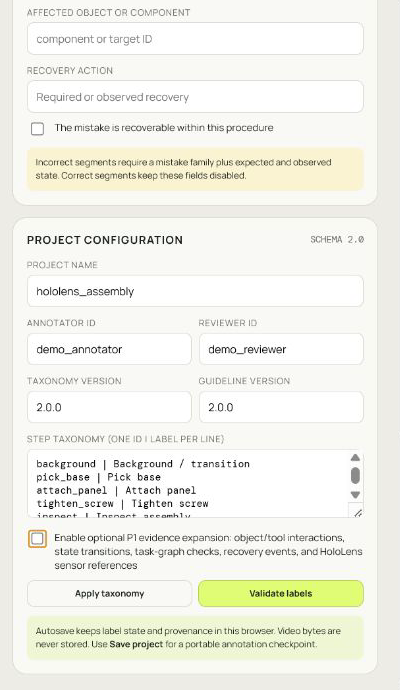
\includegraphics[height=0.34\textheight]{procedure_04b_p1_disabled.png}
  \caption{P1 disabled: the P0 project remains usable.}
\end{subfigure}
\caption{The optional expansion is controlled at project level and should be
enabled only when its evidence can be labeled consistently.}
\label{fig:p1}
\end{figure}

\section{Annotation and export contract}

\begin{table}[H]
\centering
\caption{Minimum decisions for each supervision channel.}
\small
\begin{tabularx}{\textwidth}{@{}p{0.18\textwidth}p{0.28\textwidth}Y@{}}
\toprule
\textbf{Channel} & \textbf{Required content} & \textbf{Operational rule}\\
\midrule
Capture (P0) & participant, session, split, timing and versions &
Use stable non-identifying IDs; split at participant/session level.\\
Action (P0) & class, start, end, status, confidence &
Label the smallest complete unit; boundaries follow observable motion/effect.\\
Mistake (P0) & family, severity, expected/observed state, object, recovery &
Use \code{incorrect} only when evidence contradicts the objective; otherwise use
\code{unknown} or \code{aborted} as defined.\\
Hand (P0) & PTS, handedness, 21 points, visibility, source, reviewer &
Inspect proposals and mark unlocalizable joints invisible rather than guessing.\\
Evidence (P1) & interval, type, object/tool/contact, state/effect &
Permit overlap; disable P1 when coverage cannot support the target model.\\
\bottomrule
\end{tabularx}
\end{table}

\begin{table}[H]
\centering
\caption{Schema 2.0 training-bundle artifacts.}
\small
\begin{tabularx}{\textwidth}{@{}p{0.40\textwidth}Y@{}}
\toprule
\textbf{Artifact} & \textbf{Purpose}\\
\midrule
\code{annotations/project.json} & Canonical project and preserved label state.\\
\code{metadata/capture\_manifest.csv} & Capture identity, split, dimensions,
duration, timing policy, and optional stream references.\\
\code{annotations/temporal\_manifest.jsonl} & One completed temporal record per video.\\
\code{annotations/step\_segments.csv} & Flat action and structured-mistake table.\\
\code{annotations/hand\_keypoints.csv} & One row per joint with PTS and provenance.\\
\code{annotations/coco\_hand\_keypoints.json} & COCO-style keypoint records
\cite{lin2014coco}.\\
\code{splits/\{train,val,test,exclude\}.txt} & Reproducible split membership.\\
\code{configs/procedure.json}, \code{dataset.yaml} & Taxonomy, task graph, and
training configuration.\\
\bottomrule
\end{tabularx}
\end{table}

\section{Step-by-step labeling procedure}

\subsection{Prepare, import, and configure}

\begin{enumerate}[label=\textbf{Step \arabic*.},leftmargin=4.2em]
  \item \textbf{Inventory and preserve.} Assign participant, session, task, take,
  device, and stream IDs. Retain immutable sources, checksums, time base,
  firmware, calibration, and stream inventory.
  \item \textbf{Complete privacy review.} Confirm consent, use, retention,
  access, and required face, screen, document, badge, or audio redaction
  \cite{grauman2022ego4d,ego4d_privacy}.
  \item \textbf{Create an annotation proxy.} Use a broadly decodable codec
  without replacing the original; retain proxy-to-source PTS mapping.
  \item \textbf{Freeze the guideline.} Publish class definitions, boundaries,
  examples, mistake rules, and review policy.
  \item \textbf{Import or relink.} Use \emph{Import videos}, \emph{Import
  folder}, or \emph{Import ZIP}; confirm duration, decode, and content.
  \item \textbf{Enter capture identity.} Fill participant, session, split,
  nominal frame rate, and source time base.
  \item \textbf{Enter provenance.} Fill annotator/reviewer and taxonomy/guideline
  versions, apply the versioned taxonomy, and save a portable checkpoint.
\end{enumerate}

\begin{figure}[H]
  \centering
  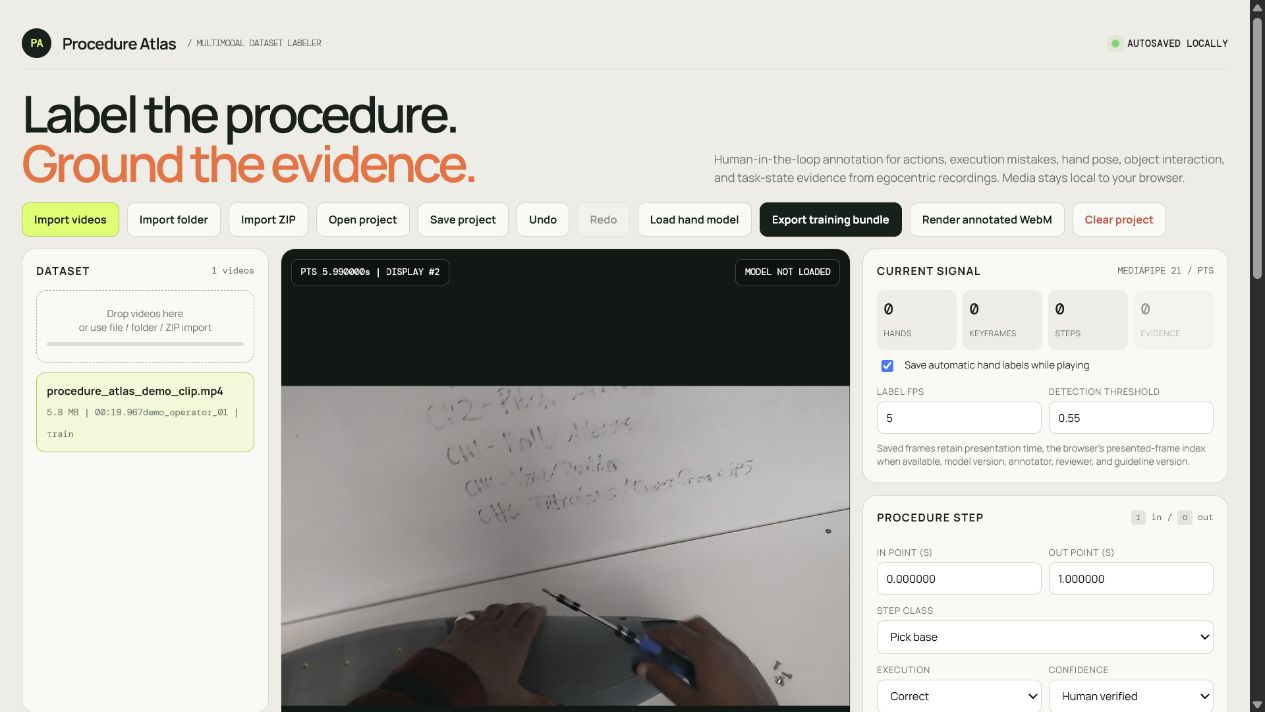
\includegraphics[width=\textwidth]{procedure_01_dataset_import.png}
  \caption{A 20-second proxy from
  \code{20260716\_012249\_HoloLens.mp4} loaded with P0 capture identity and train
  split assignment. Source footage remains local.}
  \label{fig:import}
\end{figure}

\subsection{Label hands, actions, and mistakes}

\begin{enumerate}[label=\textbf{Step \arabic*.},leftmargin=4.2em,start=8]
  \item \textbf{Load the hand model.} A failed model load is a processing
  failure, not evidence of absent hands.
  \item \textbf{Generate and review hand proposals.} Play with automatic capture
  enabled. Pause at contact, blur, occlusion, grasp change, or handedness
  uncertainty; correct joints and visibility and save the reviewed frame.
  \item \textbf{Mark an action.} Set \emph{In} at the first task-directed motion
  and \emph{Out} at the first frame after the observable effect. Select class,
  execution, and confidence, then add the segment.
  \item \textbf{Ground a mistake.} Record controlled family and severity, the
  expected state, observed contradictory evidence, affected object, and
  recovery. Do not infer hidden intent.
  \item \textbf{Keep recovery separate.} End the failed interval when its
  evidence ends; label later recovery as its own action and optional P1 event.
\end{enumerate}

\begin{figure}[H]
  \centering
  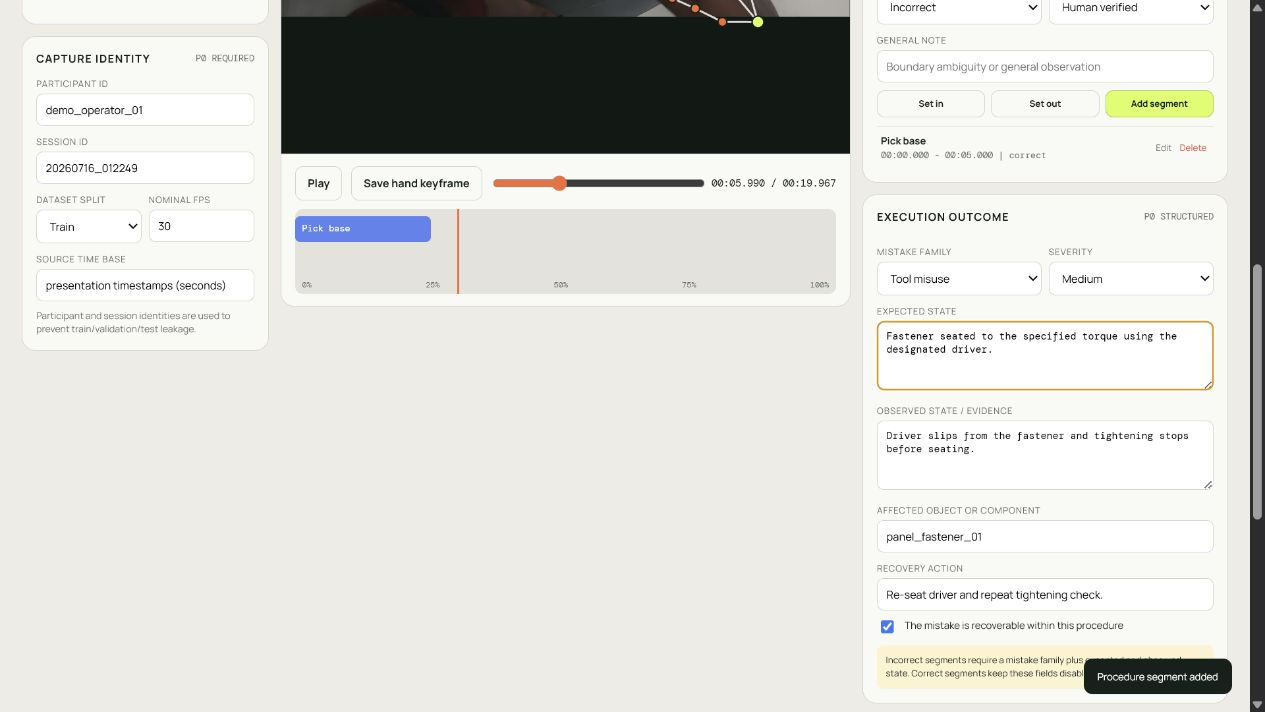
\includegraphics[width=0.93\textwidth]{procedure_03_structured_mistake.png}
  \caption{Structured P0 mistake entry for an illustrative \emph{Tighten screw}
  segment. These fields are machine-readable. The example has not been
  adjudicated as ground truth for the recording.}
  \label{fig:mistake}
\end{figure}

\subsection{Optional P1, validation, and export}

\begin{enumerate}[label=\textbf{Step \arabic*.},leftmargin=4.2em,start=13]
  \item \textbf{Decide whether P1 is supported.} Enable it only when required
  object, state, recovery, or synchronized-stream evidence can be labeled
  consistently; otherwise leave it disabled.
  \item \textbf{Add overlapping evidence.} Record interval, type, object, tool,
  contact, pre-state, post-state, expected effect, observed effect, confidence,
  and note. Add optional stream references without claiming they were decoded.
  \item \textbf{Validate.} Resolve every error and disposition warnings for
  background, class coverage, optional sensors, and missing source indices.
  \item \textbf{Review semantically.} Schema validation does not prove boundary,
  mistake, hand, or state correctness. Independently review all test errors and
  a risk-weighted sample of other labels.
  \item \textbf{Export and checksum.} Record bundle, source and proxy, app and
  schema, taxonomy and guideline, annotator and reviewer, and review date.
\end{enumerate}

\begin{figure}[H]
  \centering
  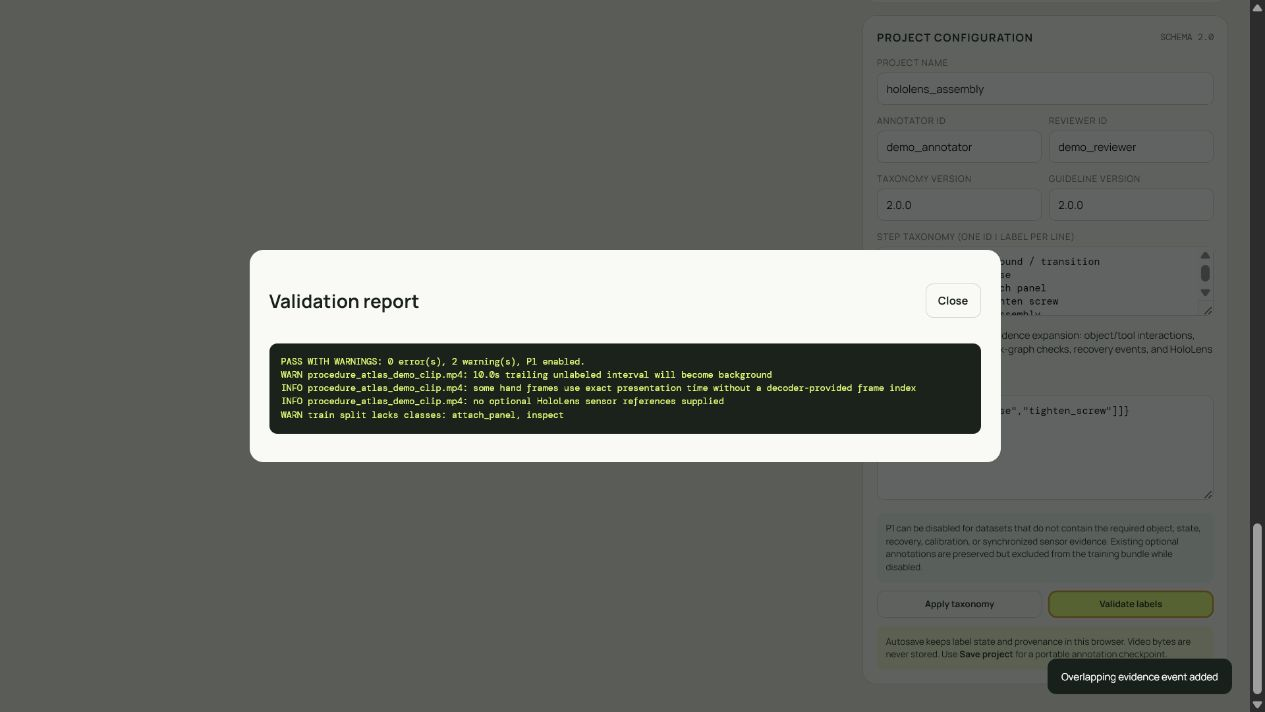
\includegraphics[width=0.83\textwidth]{procedure_05_validation.png}
  \caption{Validation reports zero errors while exposing actionable warnings
  and information: background duration, incomplete class coverage, missing
  decoder-provided frame indices, and absent optional HoloLens references.}
  \label{fig:validation}
\end{figure}

\section{Quality assurance and release gates}

Independent review should oversample mistakes, rare steps, fast motion,
occlusion, contact, and P1 events. Disagreements are adjudicated against the
guideline and converted into new examples. Guidelines and inter-annotator
agreement are coupled design problems \cite{caselli2012temporal}.

\begin{table}[H]
\centering
\caption{Recommended release gates; task risk may require stricter values.}
\small
\begin{tabularx}{\textwidth}{@{}p{0.30\textwidth}p{0.20\textwidth}Y@{}}
\toprule
\textbf{Gate} & \textbf{Target} & \textbf{Meaning}\\
\midrule
Decode and identity & 100\% & Every source opens and has stable identity/timing.\\
Validation errors & 0 & Schema, timing, taxonomy, provenance, split, and graph pass.\\
Boundary agreement & median 0.25--0.50 s or better & Reviewers place comparable boundaries.\\
Mistake double-review & 100\% of test errors & Evaluation error claims are verified.\\
Hand audit & hard frames plus sampled baseline & Blur, contact, and visibility are reviewed.\\
Participant/session leakage & 0 & Evaluation represents unseen operators/sessions.\\
P1 completeness, if enabled & predefined target & Optional coverage supports the intended model.\\
Provenance & 100\% & Sources, labels, versions, and review history are linked.\\
\bottomrule
\end{tabularx}
\end{table}

\section{Current limitations and required next work}

P0/P1 schema 2.0 closes earlier gaps: controlled mistake fields, identity and
review provenance, leakage checks, PTS/frame distinction, resumable projects,
and parallel evidence. The following limitations remain material.

\begin{table}[H]
\centering
\caption{Residual limitations affecting training readiness.}
\small
\begin{tabularx}{\textwidth}{@{}p{0.08\textwidth}p{0.30\textwidth}Y@{}}
\toprule
\textbf{Priority} & \textbf{Limitation} & \textbf{Required response}\\
\midrule
\priority{P0} & Source-to-proxy integrity is external. &
Add source/proxy hashes, PTS mapping, capture-manifest import, and bundle checks.\\
\priority{P0} & Semantic correctness/agreement are not automated. &
Add adjudication state, disagreement workflow, boundary metrics, and review reports.\\
\priority{P0} & Coverage warnings are coarse. &
Add duration/count/mistake dashboards by participant, session, class, and split.\\
\priority{P0} & Browser decoding lacks an authoritative source frame index. &
Integrate a decoder/manifest mapping; keep the index null until authoritative.\\
\priority{P1} & Sensor fields are references, not calibrated synchronized data. &
Add stream ingestion, clock-drift estimation, calibration/pose validation, and
synchronization quality metrics.\\
\priority{P1} & Objects and contacts lack spatial geometry. &
Add reviewed tracks, boxes/masks, stable object instances, and contact location.\\
\priority{P1} & Hand depth is relative 2.5D, not metric 3D. &
Fuse calibrated depth/pose and record coordinate frames and uncertainty.\\
\priority{P1} & No central multi-user audit service exists. &
Add access control, record locking, immutable revisions, and adjudication queues.\\
\bottomrule
\end{tabularx}
\end{table}

MediaPipe proposals also remain vulnerable to blur, gloves, unusual viewpoints,
self-occlusion, and tool contact. P1 is therefore an expansion path, not a claim
that all multimodal requirements are already supported.

\section{Reproducibility and training-readiness checklist}

\begin{verbatim}
dataset_root/
  raw/<participant>/<session>/<stream files>
  proxies/<participant>/<session>/<recording>.mp4
  calibration/<device>/<calibration version>/
  labels/<schema>/<taxonomy>/<export timestamp>/
  splits/{train,val,test,exclude}.txt
  metadata/capture_manifest.csv
  docs/{annotation_guideline,datasheet,consent_protocol}
\end{verbatim}

The manifest should record source/proxy checksums, PTS mapping, identity, device,
stream, frame rate/time base, calibration, consent/redaction, and exclusion
reason. Publish a datasheet covering motivation, composition, collection,
preprocessing, intended use, distribution, and maintenance
\cite{gebru2021datasheets}. Before training, verify that all errors are resolved;
warnings are dispositioned; splits are participant/session-disjoint; test
mistakes are adjudicated; unknown labels and invisible joints are masked;
background is reviewed; COCO video/PTS references are materialized for
image-only trainers; \code{z\_rel} is not treated as metric depth; and P1 is
disabled whenever its required evidence is incomplete.

\section{Conclusion}

Procedure Atlas provides a coherent P0 workflow for turning HoloLens RGB
recordings into auditable temporal actions, structured execution outcomes, and
reviewed 21-joint hand poses. Optional P1 evidence can extend this baseline
without weakening it. The interface and validator are necessary but not
sufficient: training readiness still depends on immutable source/proxy mapping,
semantic review, leakage-resistant splits, coverage analysis, privacy controls,
and---for multimodal or 3D objectives---calibrated synchronization and spatial
annotation.

\begin{thebibliography}{9}
\bibitem{microsoft_research_mode}
Microsoft. \newblock HoloLens Research Mode. \newblock Microsoft Learn, 2022.
\newblock \url{https://learn.microsoft.com/en-us/windows/mixed-reality/develop/advanced-concepts/research-mode}.

\bibitem{zhang2020mediapipe}
F. Zhang et al. \newblock MediaPipe Hands: On-device real-time hand tracking.
\newblock \emph{arXiv:2006.10214}, 2020.
\newblock \url{https://arxiv.org/abs/2006.10214}.

\bibitem{grauman2022ego4d}
K. Grauman et al. \newblock Ego4D: Around the world in 3,000 hours of egocentric
video. \newblock In \emph{CVPR}, 2022.
\newblock \url{https://arxiv.org/abs/2110.07058}.

\bibitem{peddi2024captaincook4d}
R. Peddi et al. \newblock CaptainCook4D: A dataset for understanding errors in
procedural activities. \newblock \emph{arXiv:2312.14556}, 2023.
\newblock \url{https://arxiv.org/abs/2312.14556}.

\bibitem{lin2014coco}
T.-Y. Lin et al. \newblock Microsoft COCO: Common objects in context.
\newblock In \emph{ECCV}, 2014. \newblock \url{https://arxiv.org/abs/1405.0312}.

\bibitem{caselli2012temporal}
T. Caselli et al. \newblock Temporal annotation: A proposal for guidelines and
an experiment with inter-annotator agreement. \newblock In \emph{LREC}, 2012.
\newblock \url{https://aclanthology.org/L12-1142/}.

\bibitem{gebru2021datasheets}
T. Gebru et al. \newblock Datasheets for datasets.
\newblock \emph{Communications of the ACM}, 64(12):86--92, 2021.
\newblock \url{https://doi.org/10.1145/3458723}.

\bibitem{ego4d_privacy}
Ego4D Consortium. \newblock Privacy and ethics.
\newblock \url{https://ego4d-data.org/docs/privacy/}.
\end{thebibliography}
\end{document}
